\section{Episode 65: Night on the Town}

\medskip

\textbf{Suspect Interview \#4867}\medskip

\DndDropCapLine{P}I: Name?\medskip

ES: Exmerah Danger Sliokzog\medskip

PI: Age?\medskip

ES: 7\medskip

PI: Occupation?\medskip

ES: ..errm…… gabrin\medskip

PI: …..\medskip

ES: …..\medskip

PI: Tell us in your own words about what happened again.\medskip

ES: Okay so like, we were on the airship and like, Rippy (the racist one). Rippy was wondering what all the blood was about and Myron wanted the stone of unfala that I told you about (the one that takes us to hell to talk to the elephant lady and the demon man). Myron (the mysterious one that is a bit of bad boy and you think you can probably change but also you learn a lot about yourself one) was not very tired so he asked Mr Tiger (the tiger one) to hit him and he hit him so hard he fell asleep and went to hell. Myron said that Mr Lazarus greeted him in his office and then Myron asked him all about Kiros and Mr Lazarus said he could contact her with magic. It turned out that she was asleep and Mr Lazarus said he would send Myron into her dream. In her dream she was naked but Myron said he didn’t look and also she was all bruised and crying in the corner. He lit a load of prayer candles and she said she didn’t want to speak. Also Burnie (the paedophile one) was there too.\medskip

PI: The paedophile one?\medskip

ES: Yes remember I told you he has all those files with pictures of people’s feet in. So anyway, it turned out that Kiros had been trapped in her dream for weeks! Which means it might not have even been her that we saw when she betrayed us. Myron said that she thought she might have been in the Seven Spire and that we had been seeing an imposture! Kiros had been tortured and had told them about all about us and even about excallibrum. They went back to Mr Lazarus and Burnie talked about his love of files some more. Myron woke up and told us all about how Kiros had been captured. Hmppf. I told him I prefer Arbiters that don’t get captured amirite? Anyway. Burnie pointed out that Freya had never actually disguised herself in front of us and even went so far as to say maybe Kolo might have been involved. Kolo is my brother who ripped out the spies spine and is evil now that I told you about. I was pretty sure he wasn’t capable of making a whole room of people transform into zombies.\medskip

PI: You’re referring to the entire village that you slaughtered?\medskip

ES: Yes exactly! Remember I told you that they had all been disguised as zombies by someone who wanted to trick us. Where was I? Oh yeah. Myron thought we should burn down the forest to get to Freya. Burnie invented the field of social math. Rippy pointed out that we did not even know about if Freya was a real person, which was intriguing and we knew that the mayor knew her but also fake Kiros did so who knows. Myron thought we should try and get into town and gauge public opinion. Burnie reminded everyone that we killed way more people than in Tom’ardy and Rippy started crying.\medskip

PI: Less people than Tom’ardy?!?\medskip

ES: Sorry, fewer people. But anyway, we were wondering how fake Kiros knew so much about us and suddenly we remembered that Lillith had been reporting back to Kiros on everything so that must of been how she knew! Spies everywhere! We started discussing ways to disguise ourselves to get into town. Rippy thought of maybe either shaving his beard or growing a new one underneath the current one. He also thought that we could start a questionnaire campaign and get people to send them to a PO box which is\medskip

PI: A prostitute outhouse box, yes I’m familiar.\medskip

ES: You would probably like my friend Burnie. He is a big fan of prostitute architecture as well. Burnie had a weird blank book that he asked me to look at and it turned out that there was a strong powerful magic residue left in it. Mr Tiger thought it would have been transforming magic. Turns out that the text that was there was gone and it was probably some kind of weird remote spell and someone did magic to remove the writing. Very odd. I knew it was powerful but nothing more. Myron thought we should go back and we knew that we had to do it to help people and make sure that no-one else died. We headed back to town to find out more information. Burnie went off to write a letter to Lillith. We discussed whether or not she was a spy. Rippy suggested we give up so he could go be a good father. I asked him how his children were and he said he did not even know where they were. Mother always said an absent father is a strong father. Character building. Rippy followed that up with a kidnapping idea. I volunteered to go down into town and gather information.\medskip

PI: Okay. This is when you claim to have ‘been invisible’\medskip

ES: Yes like I said I used the magic cube that we got from the old wizard in the tower full of ghosts and snake people. Rippy made the point that we might not even know who was real or not real. This was a good point but Myron said sometimes you just gotta accept stuff and get on with things. And also he pointed out that the cube could make me fly\medskip

PI: Fly?\medskip

ES: Yes. I’m not sure what you are not getting about this cube. Right so Rippy gave me a friendly push off the edge of the airship and I started falling to the ground and turned invisible on the way down and used a new thing I made which is a like blanket that makes you slower when you’re falling. I hit the ground and dumped the blanket. I was just outside Golding’s Bay. We send the poor gabrin over-board, the last thing I see is a smile and a wink as she falls backwards off the edge of the ship and down into the clouds below.\medskip

PI: Mr Tiger\medskip

T: Actually it’s Tigerius.\medskip

PI: As you wish. Please describe what happened once Exmerah got into the village.\medskip

T: Exmerah heads into town a small small gabrin in a wide and wondrous world, that without a doubt would kill and dismember her if she was ever seen. Fortune shone bright on her this day though as she was fully transparent, so in many ways fortune shone right through her which was much more beneficial.\medskip

She comes across a pile of bullet ridden metal, Stanri her lost bear. A figment of her fevered imagination when she was a child, who was briefly a hulking behemoth of a bear. More machine now than bear the animal went down shielding its master, a good boy if ever there was one. She pulls out the memory cards and gently says goodbye before heading towards the church. Candles flicker in the back as few towns folk are seen mopping up the carnage of the last conflict, which was rather one sided in the end.\medskip

Exmerah moves on, things to do, people to see, ten leaflets to put out among the people. She finds a stable, and sheds a tear for unknown reasons before setting up a ~40minute fuse on a few rockets. Before taking the backstreets to the mayors offices, all the while listening in on the local gossip “Makes you sick, doesn’t it. That someone would do something like this. I really hope they get these people” grumble some local guards. She leaves a leaflet, cast away like the hearts of so many young gabrins.\medskip

Here Ye Here Ye, the evil cult of Sin worshippers murdered the people of Goldings Bay, with some very well drawn portraits of the whole party. A notice on the town board. She puts up three flyers and stashes the big poster, she now has a rather nice team portrait.\medskip

As she closes in she comes across Arbiter Khan, and a mystery dark man, and the mayor Farnell Green. Farnell can remain the mayor if he tows the line and reports all information about the whereabouts of our group back to the Church.\medskip

Do not take these people on yourself, they have been gifted powers from Sinn and are running amok trying to cause an insurrection against the church. This group are really bad news. He bails on the stupid conversation with the old furniture moving bluff.\medskip

On a hunch Detective Exmerah skulks into the mayors office, there is smoke in the air, and she is so taken in with the dark brooding atmosphere that she knocks over a hat stand. She clicks down the voice modulator on her helmet, and starts to put the spooks into Mayor Farnell. “You let us die!!... .. .. .. . the photo of the dead family then floats over to him, he turns a deadly shade of pale as he looks at it, before he picks up the hat stand to defend himself. “The church are using you” echoes around the room as hot urine runs down legs. “You let the church slaughter us for political gain”\medskip

“This is some BULL SHIIITT”\medskip

Exmerah tries to deftly jump out of the window, but trips on some paper work as she does. Its all the noise the Mayor needs, he swiftly brings the hat stand down on her back as she gets out the window. The feel of solid flesh under the hat stand raises some pertinent questions.\medskip

She tracks down Khan flitting between the houses as they get shabbier and shabbier on the outskirts of town. She comes across the Churches wagons, the teams seem to be packing up ready to leave. They are racking and stacking rifles and ammunition. She puts a long fuse on her remaining rockets. As she is doing so a guard spots her behind some barrels. She dabs the fuse much further down, shortening the timing considerably. “Must be some of that Sinn magic they got” “After Them” finally some competent guards she thinks as she runs off. “Look there’s tracks being formed, follow the tracks”\medskip

She hides behind a bucket, unfortunately the bucket isn’t as big as she is. The guards are genuinely good at this, and follow the tracks to behind the bucket where he stabs wildly, the wee lass gasps and ducks just in time. She kicks the bucket one way, and runs the other way. There is a lot of decking in this town she thinks, and so desperately scrabbles up the side a wooden house. She looks down on the guards, and is relieved as confusion seems to spread. From the vantage point of the top of the house, she gets her bearing and locates the forest. A stable ignites in the distance as she fumbles the cube and everything slows down to a snails pace around her. This is not the flying experience she was hoping for.\medskip

She leaps down off the house and makes a run for, as she sprints past a guard she goes to pants him but her inexperience in the boudoir means she starts to fumble with the belt. She high tails it out as fast as possible out of the town. Time kicks back into its normal routine as a guard spots her, and the chase resumes. The gabrins figure blurs as she sprints into the distance, the guards raise their shotguns and unleash a hail of pellets, one of which clips her in the heel as she flees.\medskip

ES: So then like I’m running as fast as I can half full of bullets and there’s no sign of the airship. So many church soldiers behind me. Suddenly I see a blur up above me. It turns towards me and what looks like a tiger falls out of it attached to a rope then stops in mid air and goes still. Apparently Burnie had saw me and Mr Tiger had jumped off on his grappling hook to try and save me. So brave. I wondered who was driving the airship. It didn’t matter, the airship turned towards me again. A handsome shaped figure slid down the rope and landed hard on the tiger shape then went still. I carried on running. The soldiers carried on shooting but Mr Tiger started firing back. I took another spalrge of bullets as I activated my jump boots\medskip

PI: Jump boots?\medskip

ES: I told you they are the flying shoes that make you fly a little bit. Anyway, Mr Tiger caught me and Burnie started pulling us up. We got onto deck and Myron asked us what I saw. His hands were all burned from the rope. I got some vodka and cleaned them up while I told everyone what I had learned. Rippy enquired about the flyers and I told him I had handed them out and lied about also giving out the pre paid envelopes. Burnie revealed that First Mate Stick had been flying all along. I was so wrong about him and I went up to apologise to him and make amends. He stared back in a forgiving manner. Burnie took over the flying while we got rested up. I showed everybody our poster but Burnie was not happy about the quality of his drawing. Cult of Synne. Got a ring to it actually. Rippy hoped it didn’t affect our share value.\medskip

ES: We set off and I spent some time bandaging up Myron and Mr Tiger. As we flew over the world Mr Tiger told me all the things about trading and ekonomiks and he told me other things too. He told me about the animals, and showed me the strange scribbles he had made in the boat railing. The writing disappeared and a little beautiful bird came to him. Amazing. Myron shot the bird and ruined the moment a little bit but Mr Tiger continued. Burnie shouted something really weird about getting his own surrogate daughter. He and I have very different impressions of our relationship. When I turned back, Mr Tiger had gone…\medskip

PI: And that’s when you claim to have returned to hell?\medskip

ES: Yes. We fell asleep and woke up in Mr Lazarus’ office. Elephants are female mammoths. Mr Lazarus was lost for words and seemed flustered. He told us that he gets his information from people who die when they come in to hell. He said that he didn’t quite understand but some people who have died recently, well, their souls just didn’t exist anymore. Burnie asked the question. Are they really dead? Lazarus was audibly confused. Myron asked what could be done with souls. Mr Lazarus thought he had a way of tracking souls through some old equipment but he couldn’t find them anywhere. Either the souls were being destroyed or they were going somewhere beyond Mr Lazurus’ knowledge. He still could not find much on Kalimar either except for vague riddles. Apparently, the death numbers were not matching up. The theory: someone is stealing souls. Mr Tiger offered his talents as an accountant to look for trends or oddities in the soul records from the last 100 years. Necronomics. Myron asked how many people from the church had arrived. They should have gone to heaven but all came here. Myron says he is going to start making records of who we kill. We came up with a plan. We need to go to the Spires.\medskip

\textbf{Epilogue}\medskip

Tigerius walked in through the front door and took in the depravity all around him. The whores desperately trying to drum up business with the men who were now too drunk to say no. The fight in the corner, surely over nothing more sinister than a glance in the wrong direction. The fire burning low with a group of flea ridden mutts desperately trying to get a glimpse of warmth before the barkeep threw them out. The whole place stank of stale ale and shame. Over at the far side of the bar he saw the little goblin figure surrounded by a pile of empty bottles. As he got closer he heard her shouting at no-one in particular, gesturing towards the wall. “Yesh i tolds you didn’t i like invishible i was there and theey cudnt even sseemme”. He walked over. “Now now little one. What’s going on here?” he asked in his kindest tone. The little goblin girl turned towards him, here eyes bloodshot and full of tears. “I wash jhust telling the inspektor here. I wash telling him about wat reaaly happened”. He could smell the alcohol from three feet away. “I ddin’t mean to do it” she said softly. “I dddint know”. The tears came faster now as she lay her head on the bar and started sobbing. Tigerius picked her up gently in his big tiger arms. “Hush now little one. Everything’s going to be okay” he purred. She had fallen asleep, the tears drying on her face and clothes. Tigerius placed some coin onto the bar next to a poorly drawn picture of a young family that was stained with tears and left.\medskip

\vspace*{5mm}

\begin{center}
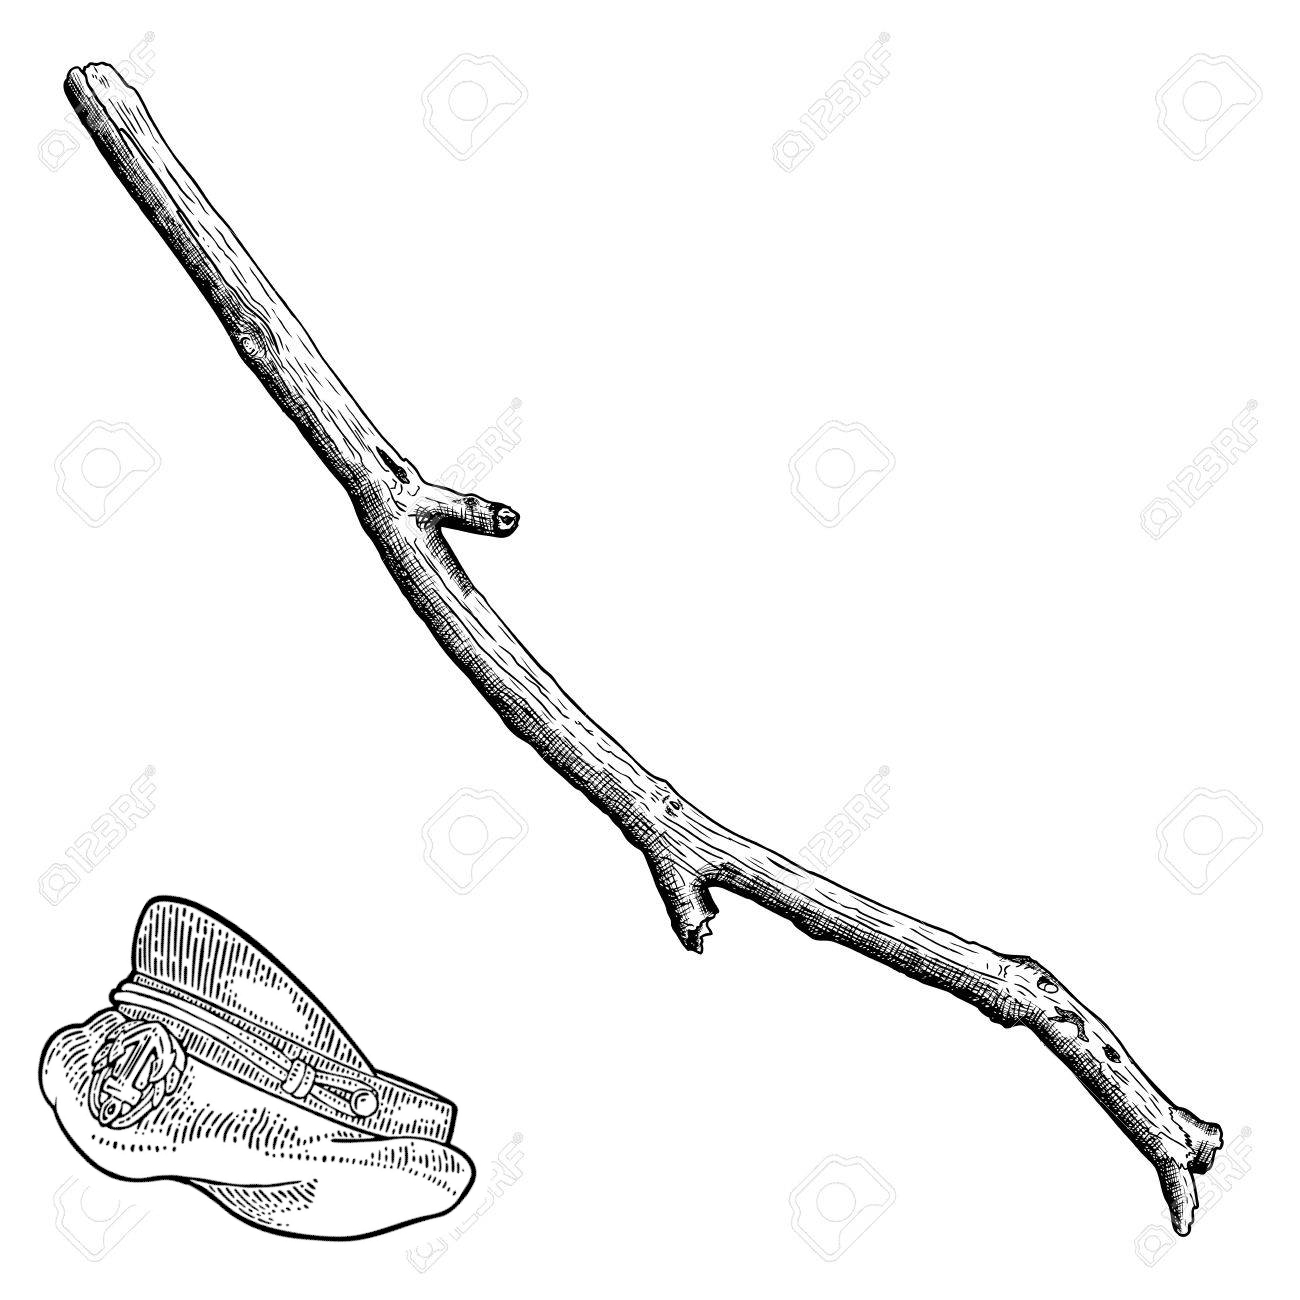
\includegraphics[width=\textwidth]{./content/img/xxx.jpg}
\begin{figure}[h]
\end{figure}
\end{center}

\clearpage
